\documentclass[11pt]{article}

\usepackage[T1]{fontenc}
\usepackage{geometry}
\usepackage{amsmath, amssymb, amsthm}
\usepackage{listings}
% \usepackage{courier}
\usepackage{xcolor}
\usepackage{graphicx}
\usepackage{fancyhdr}
\usepackage{lipsum}
% \usepackage{subfigure}
\usepackage{caption}
\usepackage{subcaption}
\usepackage{float}

\makeatletter
\renewcommand\@biblabel[1]{}
\renewenvironment{thebibliography}[1]
     {\section*{\refname}%
      \@mkboth{\MakeUppercase\refname}{\MakeUppercase\refname}%
      \list{}%
           {\leftmargin0pt
            \@openbib@code
            \usecounter{enumiv}}%
      \sloppy
      \clubpenalty4000
      \@clubpenalty \clubpenalty
      \widowpenalty4000%
      \sfcode`\.\@m}
     {\def\@noitemerr
       {\@latex@warning{Empty `thebibliography' environment}}%
      \endlist}
\makeatother

\captionsetup[table]{skip=10pt}

\geometry{a4paper, margin=1in, headheight=14pt}

\pagestyle{fancy}
\renewcommand\headrulewidth{0.4pt}
\fancyhead[L]{\scshape Experiment I}
% \lhead{Experiment I}
\rhead{}
\cfoot{\thepage}

\definecolor{darkgreen}{rgb}{0.2, 0.6, 0.4}
\definecolor{darkblue}{rgb}{0.2, 0.4, 0.8}
\lstset{ 
  basicstyle=\footnotesize\ttfamily,
  commentstyle=\color{gray},
  % extendedchars=true,
  % keepspaces=true,
  keywordstyle=\color{darkblue},
  % numbers=left,
  % numbersep=5pt,
  % numberstyle=\tiny\color{gray},
  stringstyle=\color{darkgreen},
  tabsize=4,
  % frame=lines,
  aboveskip=2em,
  belowskip=2em
}

\newcommand\pp[2]{\frac{\partial #1}{\partial #2}}

\title{
        \Large\textsc{PH2103: Physics Laboratory III} \\
        \vspace{10pt}
        \Huge \textbf{Diffraction and Interference} \\
        \vspace{5pt}
        \large{Single slit diffraction and Young's double slit experiment.}
}
\author{
        \large Satvik Saha%
        \thanks{Email: \tt ss19ms154@iiserkol.ac.in}
        \\\textsc{\small 19MS154}
}
\date{\normalsize
        \textit{Indian Institute of Science Education and Research, Kolkata, \\
        Mohanpur, West Bengal, 741246, India.} \\
        \vspace{10pt}
        \today
}

\begin{document}
        \maketitle

        % \renewcommand{\abstractname}{Aims}
        \begin{abstract}
                In this experiment, we study the phenomenon of diffraction and interference of waves, specifically electromagnetic waves or light.
                Here, we observe the diffraction patterns produced by coherent light passing through both single and double slit apertures,
                and explore their dependence on parameters such as the slit width and separation.
                We thus use diffraction patterns (generated by a coherent beam of known wavelength) to measure these parameters.
        \end{abstract}

        \section{Theory}
        
        Diffraction can be bluntly described as the phenomenon of bending of light over a sharp obstacle.
        A closer look reveals that this phenomenon is caused by electromagnetic waves interacting with matter, which alter its
        propagation. This redistribution of the `incident field' is in a sense a scattering phenomenon, introducing new components
        to the wave vector which in turn causes the wave to veer off track.
        This phenomenon is best observed in what is called a \textit{single slit experiment}, with an incident coherent, monochromatic
        beam of light passing through a narrow aperture. Under certain conditions, one of which is that the sizes of the aperture and
        the wavelength of the light must be comparable, we observe alternating bands of light and dark regions on a screen placed beyond
        the aperture. Note that this behaviour is very difficult to explain if light is thought of as a stream of particles, but
        sits very nicely with a wavelike model, where different waves are allowed to \textit{interfere} with one another.

        Interference is a phenomenon in which two waves superimpose, effectively acting like a new wave which is the sum of the 
        interfering ones. This phenomenon is best observed in a \textit{double slit experiment}, where two `rays' of 
        coherent, monochromatic light interact and produce \textit{interference fringes} on a screen -- alternating dark and
        light bands similar to, but not quite the same as a diffraction pattern. In reality, such an experiment will also
        include a component of diffraction (as any source of light, or slit through which light is restricted is of finite size and
        will inevitably introduce diffraction effects).

        In the following analysis, we adopt a purely geometric approach, which ignores the specifics of light-matter interactions
        as well as other phenonomena pertaining to the vector nature of light (such as polarization). Our main tool is 
        \textit{Huygen's principle}, with Fresnel's extension. We first need to define the notion of a \textit{wavefront}.
        This is simply a surface in space where all oscillations (due to the electromagnetic wave) are precisely in phase.
        Huygen's principle states that every element of an unobstructed wavefront through an aperture acts as a source of
        secondary disturbances. Thus, the net disturbance at any point in space is the superposition of all these secondary disturbances.
        Furthermore, the amplitude of the disturbance due to any secondary disturbance on the wavefront can be characterized as inversely proportional
        to its amplitude, inversely proportional to the distance, and dependent on the angle between the line joining them with the normal at
        the wavefront. Incorporating all of this, and using a \textit{far-field approximation}, we develop the \textit{Fraunh\"ofer integral}.
        \[
                E(x, y) = A(x, y) \iint_{\text{Aperture}} e^{-\frac{2\pi i}{\lambda z} (x'x + y'y)}\:dx'\,dy'.
        \]
        Here, $A(x, y)$ describes the complex amplitude of the source wave, typically of the form $E_0 e^{ikz} / z$.
        
        Our physical setup involves the passage of light through an fully transparent aperture in a fully opaque material, eventually
        striking a screen at a distance $z$ away.
        \begin{center}
                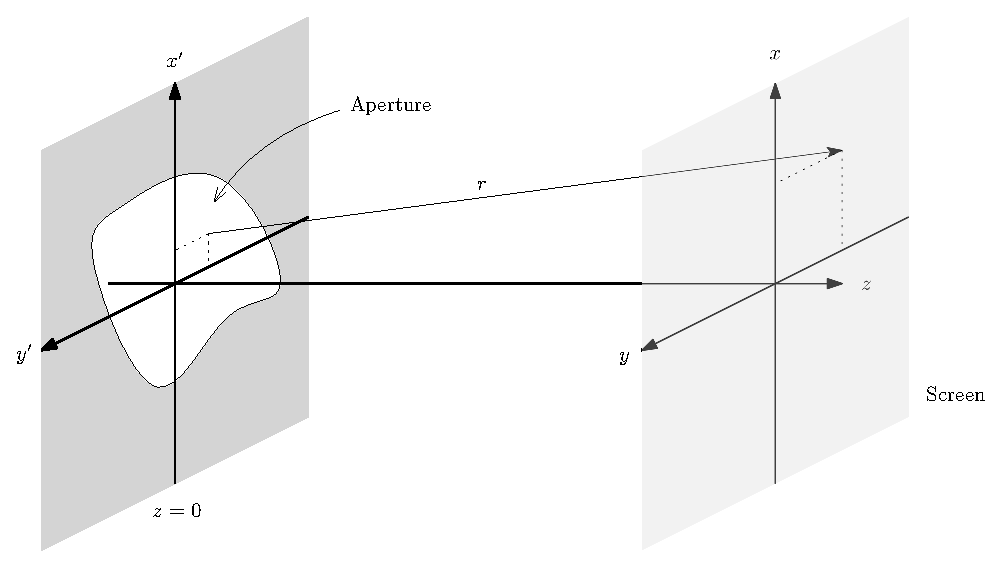
\includegraphics[scale=0.7]{fraunhofer.eps}
        \end{center}

        In the far field, where the size of the aperture $a$ through which light of wavelength $\lambda$ is allowed to pass satisfies 
        $a^2 \ll z\lambda$, we can use the Fraunh\"ofer integral to evaluate the amplitude distribution on the screen at distance $z$.
        We are of course more interested in the \textit{intensity} distribution, which is proportional to the square of the amplitude
        distribution.

        Consider the case where the aperture and screen are both one dimensional. Then we have
        \[
                E(y) = A(y) \int_{\text{Aperture}} e^{-\frac{2\pi i}{\lambda z}y'y}\:dy'.
        \]
        This integral is easily solved. The choice of the aperture determines the diffraction pattern.
        For example, a single slit of width $a$ looks like the interval $[-a/2, +a/2]$, while two such slits
        separated by a distance $d$ looks like the domain $[-(d + a)/2, -(d - a)/2]\cup [+(d - a)/2, +(d + a)/2]$.

        \paragraph{Single slit of finite width $\boldsymbol{a}$:}
        Suppose that our incident wave is a monochromatic plane wave, so $A(y) = Ae^{i\omega t}$.
        We evaluate the integral over the domain $[-a/2, +a/2]$
        \[
                E(y) = Ae^{i\omega t} \int_{-a/2}^{+a/2} e^{-2\pi i y' y /\lambda z}\:dy' =
                        -Ae^{i\omega t}\left.\frac{\lambda z}{2\pi i y}e^{-2\pi i y' y /\lambda z}\right|_{-a/2}^{+a/2}.
        \]
        Using Euler's Formula, $\sin\varphi = (e^{i\varphi} - e^{-i\varphi})/2i$, so
        \[
                E(y) =  aAe^{i\omega t}\frac{\lambda z}{\pi a y}\sin\frac{\pi a y}{\lambda z}.
        \]
        We set $y /z = \sin\theta$, where $z = D$ is the distance between the aperture and the screen.
        Since the intensity of light on the screen is proportional to $\|E\|^2$, we obtain the distribution
        \[
                I(\theta) = I_{max}\, \frac{\sin^2\alpha}{\alpha^2},
        \]
        where $\alpha = \pi a\sin\theta /\lambda$.

        Clearly, minima occur where $\sin\alpha = 0$, i.e.\ $\alpha = \pi a \sin\theta /\lambda = n\pi$ for integers $n$.
        The exception is at the very center, where we take the limit $\lim_{\alpha \to 0} \sin\alpha /\alpha = 1$, so
        $\theta = 0$ actually corresponds to a central maxima of maximum intensity (equal to the intensity of the incident beam).
        For small $\theta$, we can approximate the positions of the minima as $\theta = n\lambda /a$.
        Thus, the first minima on either side of the central maxima are at $\pm \lambda /a$. This means means that the angular width of the central maxima
        is simply $2\lambda /a$, which can be measured and used to determine the width $a$ of the slit precisely.
        If the screen is located at a distance $D$ from the slits, then $\theta \approx y /D$, so the width of the central maxima $\Delta y$
        is related to $a$ as
        \[
                a = \frac{2\lambda D}{\Delta y}.
        \]

        \paragraph{Two slits each of finite width $\boldsymbol{a}$, separated by a distance $\boldsymbol{d}$:}
        We proceed similarly as before, except we have the sum of two integrals
        \[
                E(y) = Ae^{i\omega t} \left[\int_{-(d + a)/2}^{-(d - a)/2} + \int_{+(d - a)/2}^{+(d + a)/2}\right] e^{-2\pi i y' y /\lambda z}\:dy' =
                        aAe^{i\omega t}(e^{\pi i d /\lambda z} + e^{-\pi i d /\lambda z})\frac{\lambda z}{\pi a y}\sin\frac{\pi a y}{\lambda z}.
        \]
        This time, we use Euler's Formula for the cosine, $\cos\varphi = (e^{i\varphi} + e^{-i\varphi})/2$ to obtain
        \[
                E(y) =  2aAe^{i\omega t}\frac{\lambda z}{\pi a y}\cos\frac{\pi d y}{\lambda z}\sin\frac{\pi a y}{\lambda z}.
        \]
        Like before, we set $y /z = \sin\theta$. Thus, we obtain the intensity distribution
        \[
                I(\theta) = I_{max} \cos^2\beta\, \frac{\sin^2\alpha}{\alpha^2},
        \]
        where $\alpha = \pi a\sin\theta /\lambda$ and $\beta = \pi d\sin\theta /\lambda$.
        
        Observe that for a double slit, the intensity distribution is very similar to that of a single slit of finite width,
        except with the introduction of many convolutions due to the $\cos^2\beta$ distribution of a `perfect' (zero width) double slit.

        The location of maxima and minima of the envelope remain the same as before, since the $\sin^2\alpha /\alpha^2$ form remains unchanged.
        Thus, these can be used to determine the width of the two slits like in the previous case.
        The convolutions $\cos^2\beta$ introduce finer maxima and minima.
        These minima happen when $\cos\beta = 0$, i.e.\ $\pi d\sin\theta /\lambda = (2n + 1)\pi /2$. Again, for small $\theta$, we approximate the
        positions of the minima as $\theta = (2n + 1) \lambda /2d$, which means that the first two minima occur at $\lambda /2d$ and $3\lambda /2d$.
        This angular width $\lambda /d$ between successive minima can be used to determine the separation $d$ between the two slits.
        We make the approximation $\theta \approx y /D$ to relate the separation $\Delta y'$ of successive minima with $d$ as
        \[
                d = \frac{\lambda D}{\Delta y'}.
        \]

        \newpage 
        \section{Experimental setup}
        A laser diode is used as a source of coherent monochromatic light. The wavelength of emitted light $\lambda$ is noted.
        The laser is set up on an optical bench, with a single slit in front of it.
        The laser beam is adjusted so that it is centered on the slit, and a detector is set up on the other side of the bench at the
        same height as the diffraction pattern. This detector is coupled to a rotary motion sensor, which measures the displacement of
        the detector along the axis perpendicular to the beam.
        The distance $D$ between the slit and the detector is measured and noted.
        A suitable software (\textit{Science Workshop}) is connected to the detector and the rotary motor, and is set to record data.
        The detector is slowly moved across the diffraction pattern from one end to the other.
        The data is exported to a suitable format and the procedure is repeated for three single slits and one double slit.

        \section{Experimental data and analysis}
        \subsection{Processing and plotting}
        Intensity and displacement data has been gathered and exported as Excel spreadsheets.
        The following code has been used to preprocess and visualize the raw data.
        We have used the python library \texttt{pandas} to extract data and \texttt{matplotlib}/\texttt{pyplot} to plot graphs.
        
        \lstinputlisting[language=Python]{plot.py}

        Note that the displacements measured by the rotary motor have been appropriately calibrated with actual displacements.
        Graphs of the data are presented below.

        \begin{figure}[H]
        \centering
        \begin{subfigure}[b]{0.49\textwidth}
                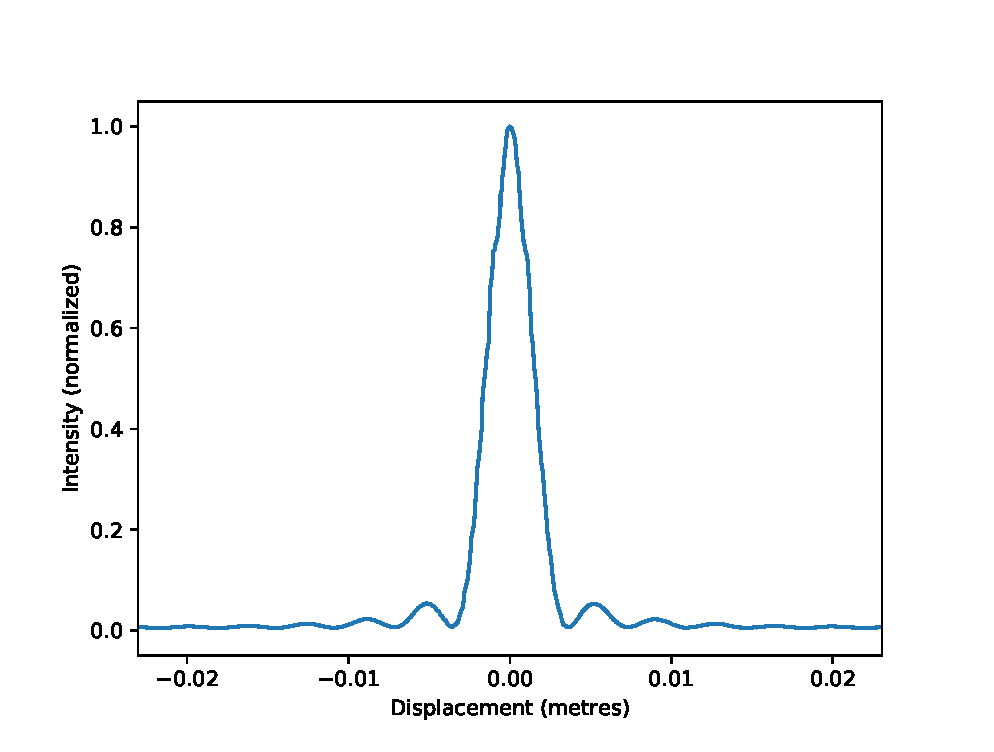
\includegraphics[width=\textwidth]{Slit1.eps}
                \caption{$D = 0.90$ m}
        \end{subfigure}
        \begin{subfigure}[b]{0.49\textwidth}
                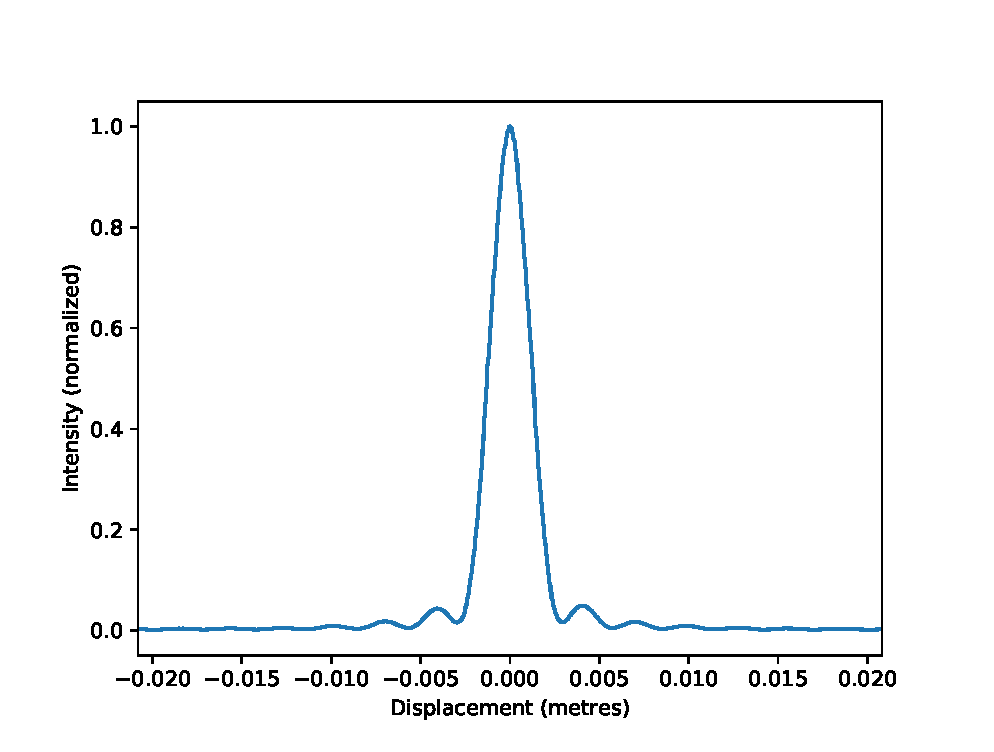
\includegraphics[width=\textwidth]{Slit2.eps}
                \caption{$D = 0.73$ m}
        \end{subfigure}
        \begin{subfigure}[b]{0.49\textwidth}
                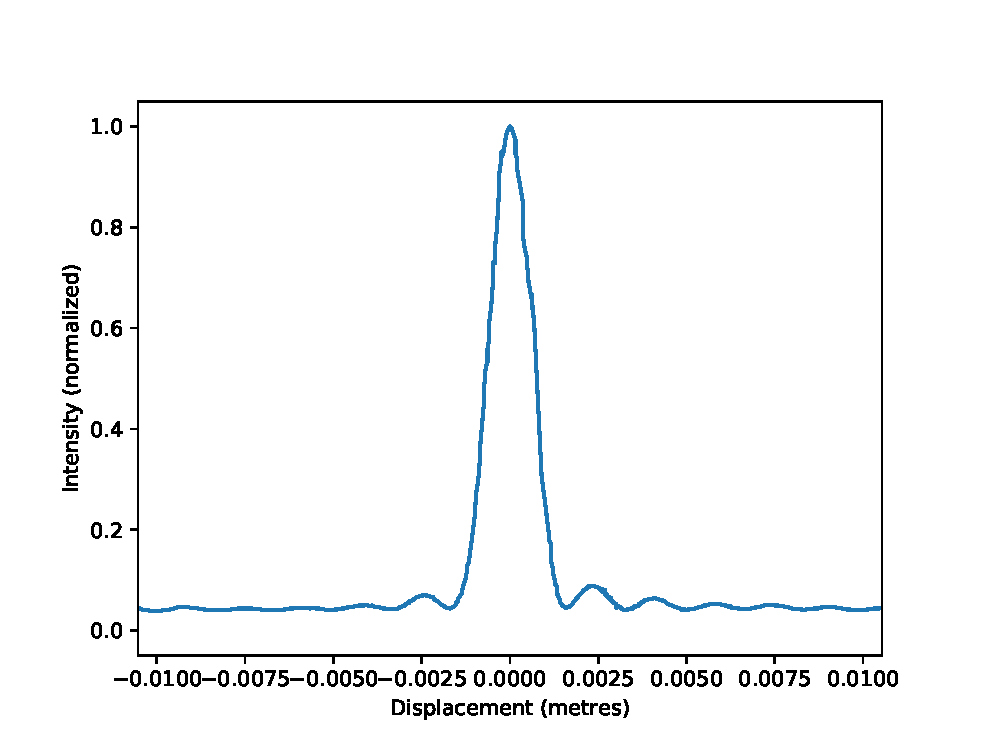
\includegraphics[width=\textwidth]{Slit3.eps}
                \caption{$D = 0.41$ m}
        \end{subfigure}
        \begin{subfigure}[b]{0.49\textwidth}
                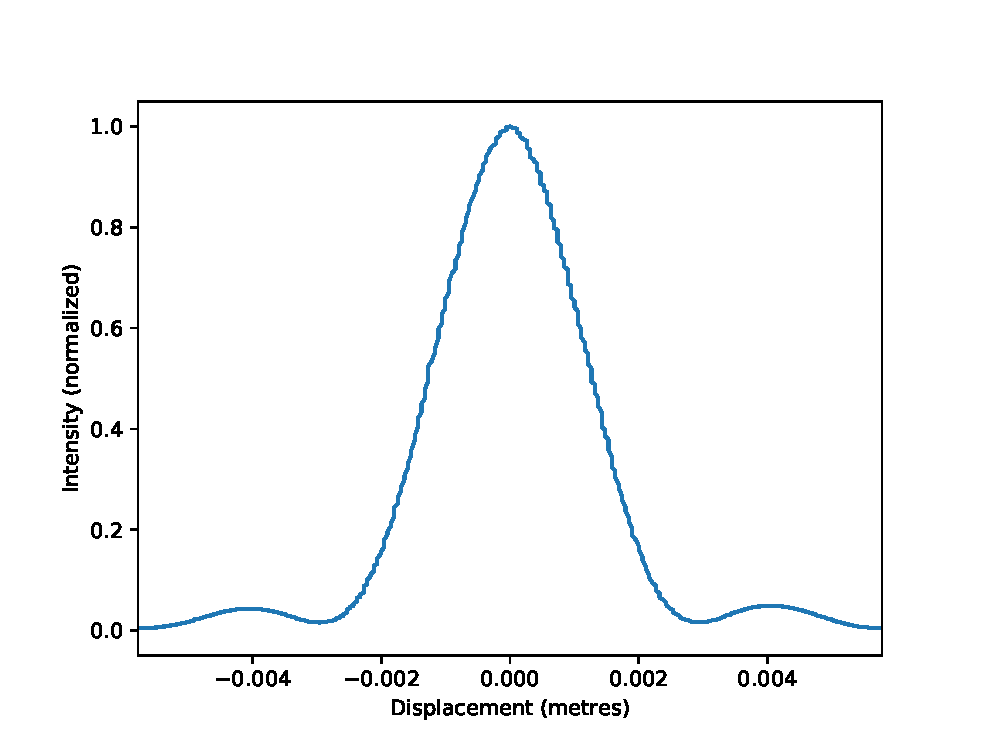
\includegraphics[width=\textwidth]{Slit2_detail.eps}
                \caption{$D = 0.73$ m, central maxima}
        \end{subfigure}
        \caption{Data from single slit measurements.}
        \label{fig:single}
        \end{figure}

        \begin{figure}[H]
        \centering
        \begin{subfigure}[b]{0.49\textwidth}
                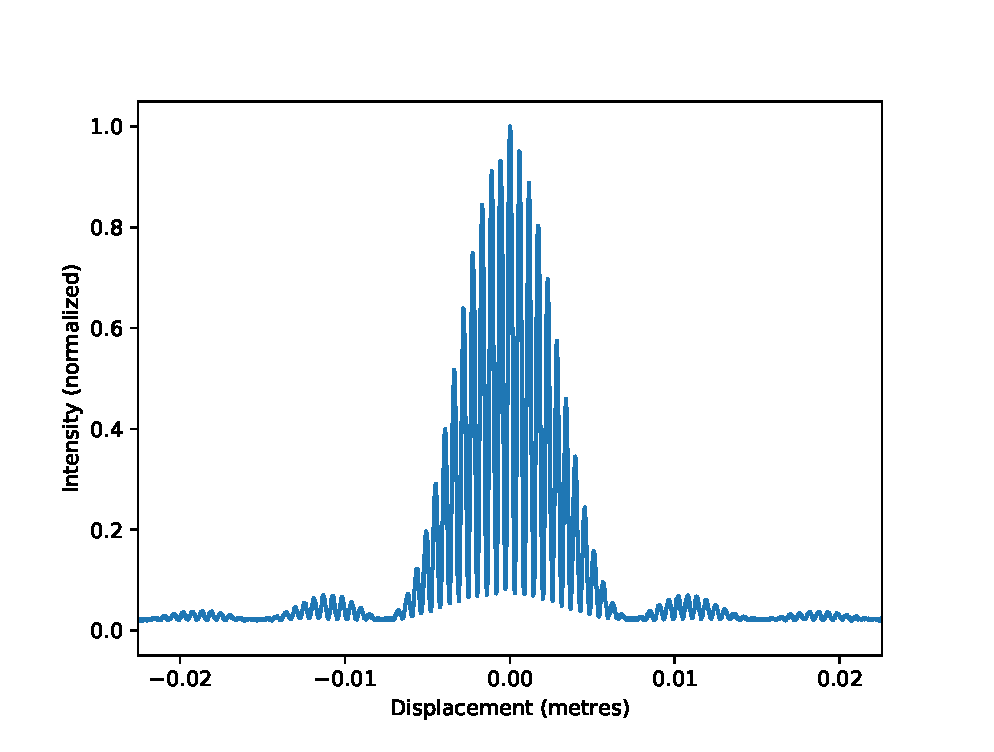
\includegraphics[width=\textwidth]{Slit4.eps}
                \caption{$D = 0.90$ m}
        \end{subfigure}
        \begin{subfigure}[b]{0.49\textwidth}
                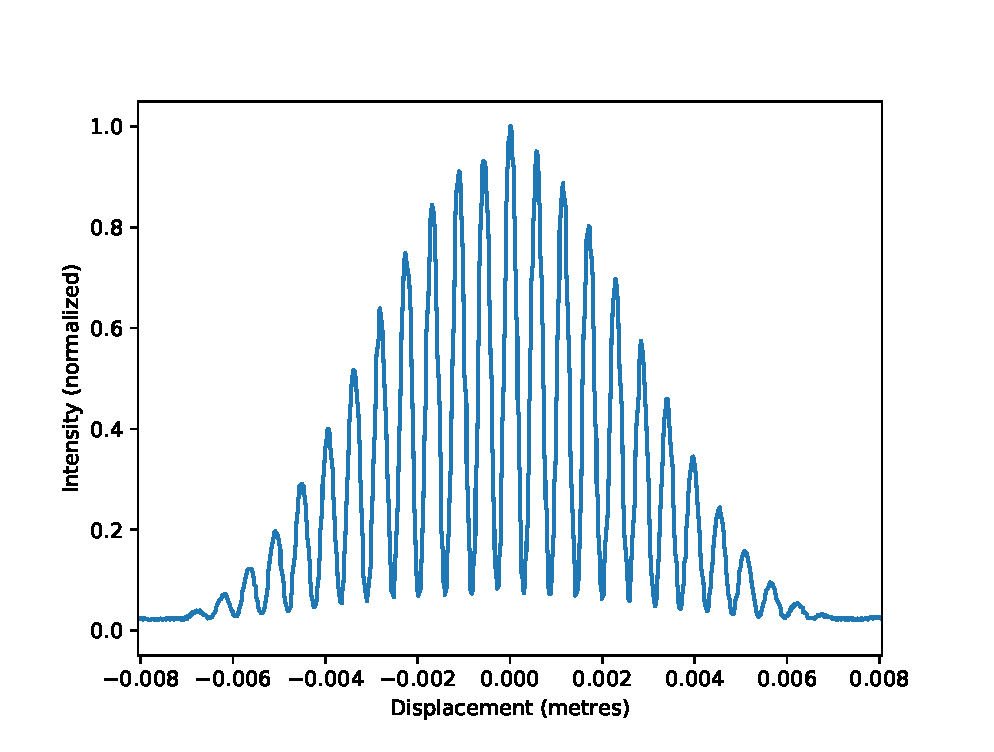
\includegraphics[width=\textwidth]{Slit4_detail.eps}
                \caption{Central maxima in detail}
        \end{subfigure}
        \caption{Data from the double slit measurement.}
        \label{fig:double}
        \end{figure}
        

        The \texttt{pyplot} interface lets us determine the precise coordinates of points on the curve, so we use this tool to calculate the
        width of the central maxima and distances between minima as required. These are tabulated below.
        We have also calculated the slit widths $a_i$ and the distance between the slits $d$ using the formulae mentioned in the theory section.

        \begin{table}[H]
                \centering
                \caption{Parameters and quantities. The wavelength of light used is $\lambda = 650 \pm 3$ nm.
                All the $a_i$ are calculated as $2\lambda D/\Delta y$ and $d$ is calculated as $\lambda D /\Delta y$.}
                \label{tab:parameters}
                \begin{tabular}{l|c|c|c|c}\hline
                Slit type       & Quantity & Distance $D$ (m)    & Separation $\Delta y$ (m)    & Value of quantity     \\\hline\hline
                                & $a_1$    & 0.90                & 0.0072                       & $a_1 = 0.000163$ m    \\
                Single Slit     & $a_2$    & 0.73                & 0.0059                       & $a_2 = 0.000161$ m    \\
                                & $a_3$    & 0.41                & 0.0033                       & $a_3 = 0.000162$ m    \\\hline
                Double Slit     & $a_4$    & 0.90                & 0.0150                       & $a_4 = 0.000078$ m    \\
                                & $d$      & 0.90                & 0.00057                      & $d =   0.00103$ m\\\hline
                \end{tabular}
        \end{table}
        
        
        \subsection{Error Analysis}
        For the quantity $a = f(Y, D, \lambda) = 2\lambda D/Y$, with standard deviations $\delta a$, $\delta Y$, $\delta D$ and $\delta \lambda$,
        we relate them using
        \begin{align*}
                (\delta a)^2 \;&=\; \left|\pp{f}{Y}\right|^2(\delta Y)^2 \,+\, 
                                        \left|\pp{f}{D}\right|^2(\delta D)^2 \,+\,
                                        \left|\pp{f}{\lambda}\right|^2(\delta \lambda)^2 \\
                        \;&=\; \left(\frac{2\lambda D}{Y^2}\right)^2(\delta Y)^2 \,+\, \left(\frac{2\lambda}{Y}\right)^2(\delta D)^2 \,+\,
                                \left(\frac{2D}{Y}\right)^2(\delta \lambda)^2.
        \end{align*}
        We note that this is equivalent to writing
        \[
                \left( \frac{\delta a}{a} \right)^2 \;=\; \left( \frac{\delta Y}{Y} \right)^2  \,+\, \left( \frac{\delta D}{D} \right)^2 \,+\,
                                \left( \frac{\delta \lambda}{\lambda} \right)^2 .
        \]
        Similarly, for $d = \lambda D/Y$, we can show that like before,
        \[
                \left( \frac{\delta d}{d} \right)^2 \;=\; \left( \frac{\delta Y}{Y} \right)^2  \,+\, \left( \frac{\delta D}{D} \right)^2 \,+\,
                                \left( \frac{\delta \lambda}{\lambda} \right)^2 .
        \]

        Note that in place of $Y$, we actually have $Y = \Delta y = y_2 - y_1$, so $(\delta Y)^2 = 2\, (\delta y)^2$.
        Also, actual displacements $y$ are related to displacements $y'$ measured by the rotary motion sensor by a scaling factor as $y = k y'$,
        where $k = 0.05 /0.0946$. Thus, $\delta y = k \,\delta y'$.

        For the single slit, we have three measurements, each with standard deviation $\delta a_i$.
        We report the (na\"ive) mean $\bar{a}$, with standard deviation $\delta a = \frac{1}{3}\sqrt{(\delta a_1)^2 + (\delta a_2)^2 + (\delta a_3)^2}$.

        We tabulate the standard deviations $\delta X$ in measured quantities below.
        
        \begin{table}[H]
                \centering
                \caption{Standard deviations in measured quantities, with justification.}
                \label{tab:deviations}
                \begin{tabular}{c|c|c|l}\hline
                Quantity        & Deviation             & Value         & Justification         \\\hline\hline
                Wavelength      & $\delta\lambda$       & 3 nm          & Given                 \\
                Distance        & $\delta D$            & 0.5 mm        & Least count of scale  \\
                Displacement    & $\delta y'$           & 0.1 mm        & Resolution of rotary sensor \\
                                & $\delta y$            & 0.05 mm       & $\delta y = k\, \delta y'$ \\
                                & $\delta Y$            & 0.075 mm      & $\delta Y = \sqrt{2}\, \delta y$ \\\hline
                \end{tabular}
        \end{table}
        
        By far the biggest source of measurement uncertainty is from the separation $\delta y$. The relative error $\delta Y / Y$ is
        on the order of $1\%$ in the single slits, only $0.5\%$ in the slit width in the double slit, but contributes nearly the whole $13\%$
        when calculating the separation of slits! In contrast, the relative errors $\delta D / D$ are usually of the order of $0.1\%$, 
        and $\delta\lambda / \lambda$ is around $0.5\%$. It may be the case that we have overestimated $\delta Y$, which we could have
        reduced by taking multiple measurements. Indeed, repeating the measurement by considering $n$ such fringe widths near the center,
        we could cut this uncertainty by $\sqrt{n}$. Considering the $14$ fringes which span $0.008$ m in the central maxima, we see that their widths 
        agree at $0.00057$ m each. Thus, we can cut down the relative error to $\delta Y / Y \approx 13 / \sqrt{14} \approx 3.5\%$.

        The standard deviations in $a_i$ and $d$ are listed below.
        \begin{table}[H]
                \centering
                \caption{Standard deviations in calculated quantities.}
                \label{tab:deviations_calculated}
                \begin{tabular}{c|c|c}\hline
                Quantity        & Deviation     & Value         \\\hline\hline
                $a_1$           & $\delta a_1$  & 1.8 $\mu$m    \\
                $a_2$           & $\delta a_2$  & 2.2 $\mu$m    \\
                $a_3$           & $\delta a_3$  & 3.7 $\mu$m    \\
                $\bar{a}$       & $\delta a$    & 1.6 $\mu$m    \\
                $a_4$           & $\delta a_4$  & 0.53 $\mu$m   \\
                $d$             & $\delta d$    & 36 $\mu$m    \\\hline
                \end{tabular}
        \end{table}
        

        \subsection{Reported Values}
        \begin{table}[H]
                \centering
                \caption{Calculated quantities with uncertainties.}
                \label{tab:calculated_values}
                \begin{tabular}{c|c|c|c}\hline
                Slit type       &Quantity                       & Reported value        & Percentage uncertainty\\\hline\hline
                Single Slit     &Slit width ($a$)               & $162.0 \pm 1.6$ $\mu$m& 1.0\%         \\
                Double Slit     &Slit width ($a_4$)             & $78.0 \pm 0.6$ $\mu$m & 0.8\%         \\
                                &Distance between slits ($d$)   & $1.03 \pm 0.04$ mm    & 4 \%          \\\hline
                \end{tabular}
        \end{table}

        \section{Discussion}
        
        \subsection{Sources of error}
        As previously discussed in the erorr analysis section, the largest contributer of error is related to the rotary motion sensor,
        which has a fairly low resolution for the measurements we are trying to make.
        Additionally, the minima are somewhat spread out, especially in the case of the double slit where the
        minima of the envelope is highly convoluted.
        This introduces a degree of random error, which is reflected in the low precision of measurements where $\Delta y$ is small.
        Other sources of random error involve the laser diode, which may not be perfectly monochromatic.

        Without knowledge of the expected values for slit widths and separation, it is difficult to judge systematic error.
        Some possible sources may be an incorrectly calibrated instrument or a tilted axis for the light sensor (if the sensor doesn't
        move exactly perpendicular to the laser beam, this would distort all displacements).
        Furthermore, the slits may not be completely identical, which leads to a phenomenon which we discuss in the next subsection.

        \subsection{Fringe visibility}
        A curious phenomenon is observed in the double slit data, where the intensity distribution seems to have a lower envelope,
        of the same form as the upper envelope, instead of the expected flat lower envelope (all minima are expected to be of zero intensity).
        \begin{figure}[H]
                \centering
                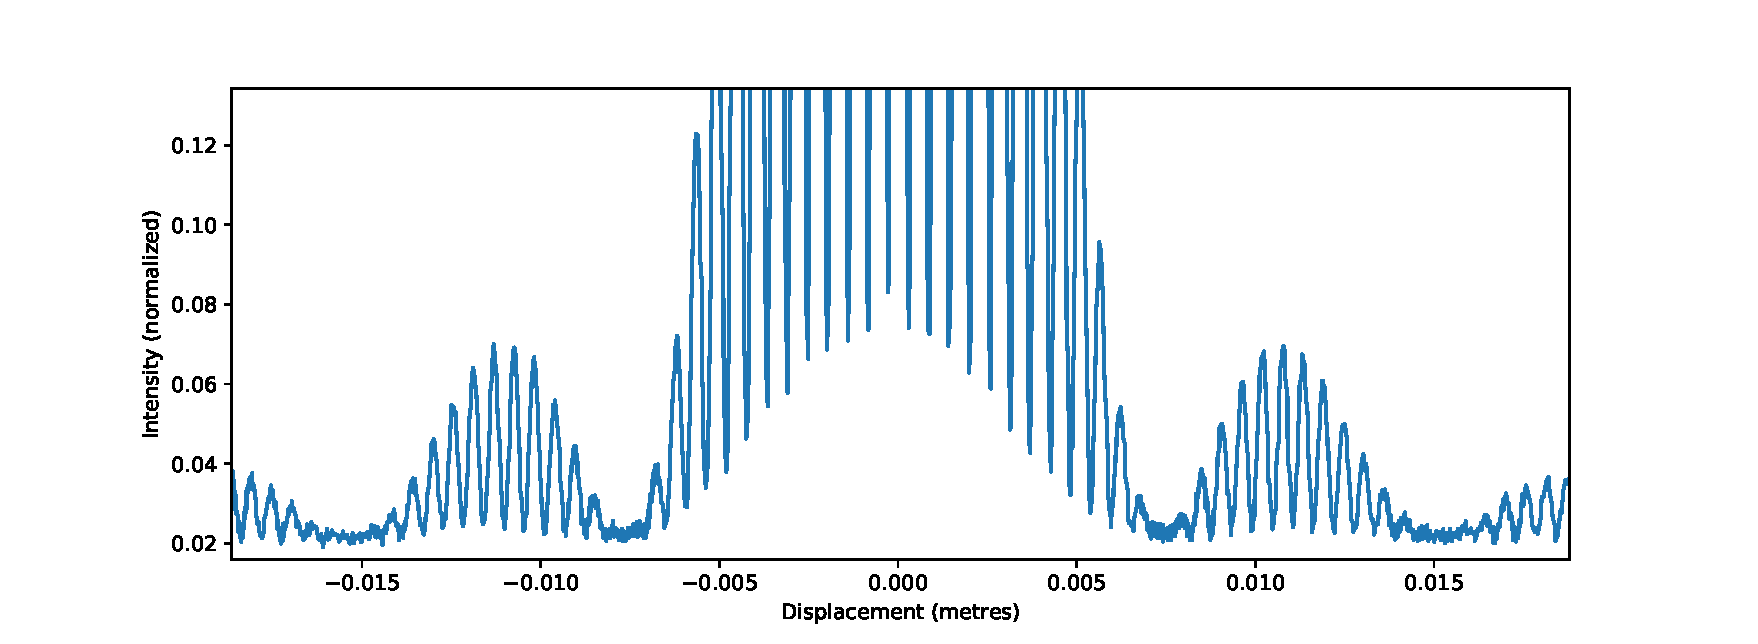
\includegraphics[width=\textwidth]{Slit4_lower.eps}
                \caption{Detail of lower half of the double slit diffraction pattern. Note the presence of a `lower envelope'.}
                \label{fig:double_lower}
        \end{figure}

        We may explain this by proposing that the two slits are not equally illuminated, perhaps due to slightly differing size
        or an asymmetric positioning of the laser. Recall that with symmetrical slits, we expected an amplitude distribution $E(y)$.
        Suppose that one of the slits is illuminated with amplitude $A_1 = (1 + \epsilon)A$, and the other slit 
        is illuminated with amplitude $A_2 = (1 - \epsilon)A$ instead.
        Using the Fraunh\"ofer integral, we thus have the new distribution $\tilde{E}(y)$, where
        \[
                \tilde{E}(y) = E(y) + \epsilon a A e^{i\omega t}(e^{i\beta} - e^{-i\beta}) \frac{\sin\alpha}{\alpha} = 
                        E(y) + 2i\epsilon aAe^{i\omega t}\sin\beta\, \frac{\sin\alpha}{\alpha}.
        \]
        To obtain the intensity profile, we square the absolute value, thus obtaining
        \[
                \| E(y) \|^2 \,+\, 4\epsilon^2a^2A^2\sin^2\beta\,\frac{\sin^2\alpha}{\alpha^2}.
        \]
        Setting $I_0 \propto 4a^2A^2$, we obtain our new intensity distribution,
        \[
                \tilde{I}(\theta) \;=\; I_0\cos^2\beta\,\frac{\sin^2\alpha}{\alpha^2} \,+\, \epsilon^2I_{0}\sin^2\beta\,\frac{\sin^2\alpha}{\alpha^2}.
        \]
        Comparing this with the older $I(\theta)$, we see that the second term clearly constitutes an additional lower envelope.
        Note that the maxima in the upper envelope is simply $I_{max} = I_0$,
        and the maxima in the lower envelope is $I_{min} = \epsilon^2 I_0$, both at $\beta = 0$.
        This is closely related to a parameter called \textit{fringe visibility}, which is calculated as
        \[
                \mathcal{V} = \frac{I_{max} - I_{min}}{I_{max} + I_{min}} = \frac{2\sqrt{I_1I_2}}{I_1 + I_2}
                        = \frac{1 - \epsilon^2}{1 + \epsilon^2}.
        \]
        Here, $I_1 \propto (1 + \epsilon)^2$ and $I_2 \propto (1 - \epsilon)^2$ are the incident intensities on the two slits.

        In our particular case, we observe that $I_{min} \approx 0.075 I_{max}$, from which we have $\epsilon \approx 0.27$ and
        $\mathcal{V} \approx 86\%$. Thus, $I_1 / I_2 \approx 3$.

        
        \section{Conclusion}
        In conclusion, we have observed the phenomena of diffraction and interference, and used them to make precise measurements
        of quantities on a microscopic scale.

        \nocite{*}
        \bibliographystyle{plain}
        \bibliography{ref}

\end{document}
